% !TeX spellcheck = it_IT
\newpage
\section{Support Vector Machine}
Il SVM è un classificatore derivato dalla \textit{teoria statistica dell'apprendimento} da Vapnik. Divenne famoso nel 1990, dopo anni di sviluppo, quando riuscì a riconoscere disegni a mano con un'accuratezza pari a reti neurali SotA.\\
Al momento è utilizzato in tutte le applicazioni di tipo \textit{Supervised} e persino nella regressione.\\
Ad oggi molte reti neurali comunque lo battono in performance.
\subsection{Maximum margin classifier}
\subsubsection{Rappresentazione}
Partiamo da un problema di classificazione binaria che sia linearmente separabile e con dati privi di rumore.
\begin{definition}[Margine]
	Dato l'iperpiano di separazione, il margine è il doppio della distanza che lo separa dai dati più vicini.
\end{definition}
Chiaramente, non tutti gli iperpiani che risolvono il problema hanno gli stessi margini:
\begin{center}
	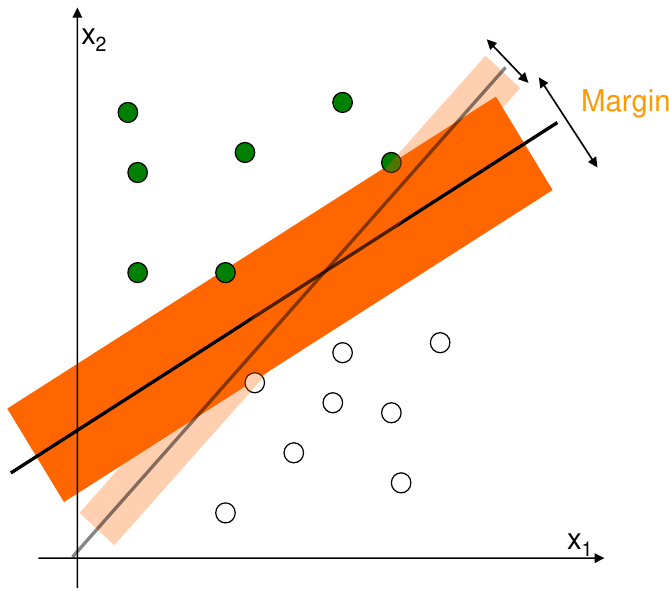
\includegraphics[scale=0.3]{svm_margin.png}
\end{center}
La rappresentazione canonica dei support vectors di un iperpiano sarà quindi:
\begin{equation}
	\mathbf{x}_p \: t.c. \: \lvert \mathbf{w}^T \mathbf{x}_p + b \rvert = 1 \quad\quad b=w_0
\end{equation}
\begin{center}
	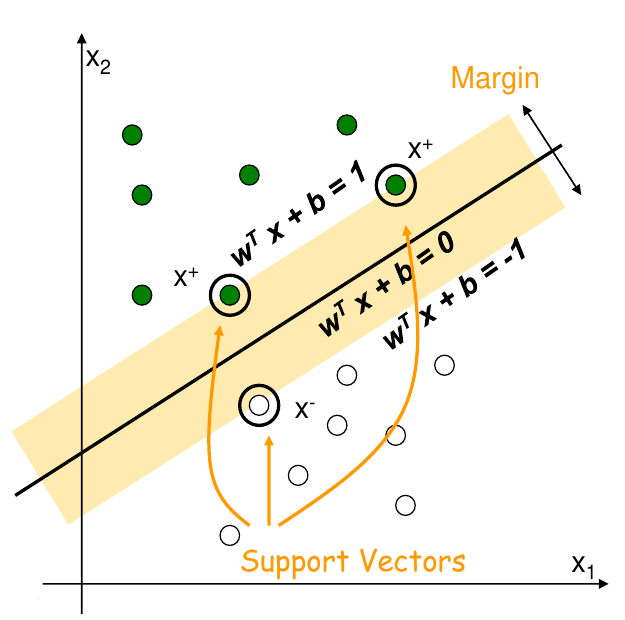
\includegraphics[scale=0.4]{svm_sv.png}
\end{center}
\subsubsection{Soluzione}
Adesso abbiamo una nuova definizione di problema di addestramento:
\begin{definition}[Training problem]
	\label{def:trainingprob}
	Vogliamo trovare $(\mathbf{w},b)$ tali che tutti i punti siano classificati correttamente e il margine sia massimizzato.
\end{definition}
I punti sono classificati correttamente se:
\begin{equation*}
	\mathbf{w}^T\mathbf{x}_p + b \geq 0 \Leftarrow y_p = 1\land \mathbf{w}^T\mathbf{x}_p + b < 0 \Leftarrow y_p = -1 \quad\quad \forall p
\end{equation*}
e possiamo adattare la definizione al margine, in modo che $\lvert \mathbf{w}^T \mathbf{x}_p + b \rvert = 1$
\begin{equation*}
	\mathbf{w}^T\mathbf{x}_p + b \geq 1 \Leftarrow y_p = 1\land \mathbf{w}^T\mathbf{x}_p + b \leq -1 \Leftarrow y_p = -1 \quad\quad \forall p
\end{equation*}
Alla fine quindi avremo i seguenti \textbf{limiti}:
\begin{equation}
	\label{eq:constraints}
	(\mathbf{w}^T \mathbf{x}_p + b)y_p \geq 1 \quad\quad \forall p
\end{equation}
Due fatti importanti per il margine:
\begin{itemize}
	\item Possiamo massimizzare il margine se e solo se minimizziamo $\lvert \mathbf{w} \rvert $ se e solo se minimizziamo $\frac{\lvert \mathbf{w} \rvert ^2}{2}$
	\begin{equation}
		\label{eq:trainprobprim}
		Margin \propto \frac{2}{\lvert \mathbf{w} \rvert} \quad\quad [\lvert \mathbf{w}\rvert^2 = (\mathbf{w}^T\mathbf{w})]
	\end{equation}
	\item \textit{VC-dim} è inverso al margine, quindi decresce quando il margine aumenta, quindi possiamo controllare la complessità del modello con il margine
\end{itemize}
\subsubsection{Quadratic optimization problem}
Visto il nuovo \hyperref[def:trainingprob]{training problem}, la sua \hyperref[eq:trainprobprim]{forma primale} e i suoi \hyperref[eq:constraints]{limiti}, ci ritroviamo con un problema di ottimizzazione quadratica.\\
Possiamo riscrivere il problema come:
\begin{equation}
	Maximize_\alpha \sum_{i}\alpha_i - \sum_{ij} \frac{\alpha_i \alpha_j y_i y_j \mathbf{x}_i^T \mathbf{x}_j}{2} \quad \quad i,j = 1, \ldots, l \quad\quad a_i \geq 0 \quad\quad \sum_{i}a_iy_i=0
\end{equation}
Vogliamo trovare gli $\alpha_p p = 1\ldots l$ ottimali (moltiplicatori di Lagrange) tramite la programmazione quadratica. Il costo computazionale aumenta con $l$ e non con $n$.\\
Possiamo ora ricavare da questa nuova riscrittura anche $(\mathbf{w},b)$:
\begin{equation}
	\mathbf{w} = \sum_p \alpha_p y_p \mathbf{x}_p \quad\quad p=1, \ldots, l \quad \quad b=y_k - \mathbf{w}^T\mathbf{x}_k \quad\quad \forall a_k > 0
\end{equation}
e quindi la funzione di approssimazione sarà:
\begin{equation}
	h(\mathbf{x})=sign(\mathbf{w}^T \mathbf{x}+b) = sign\bigg(\sum_{p=1}^{l}\alpha_py_p\mathbf{x}^T_p\mathbf{x}+b\bigg) = sign \bigg(\sum_{p\in SV}\alpha_py_p\mathbf{x}^T_p\mathbf{x}+b\bigg)
\end{equation}
Questa nuova forma della soluzione ci evita anche di dover calcolare $(\mathbf{w},b)$ in quanto è formulata solo in termini dei Support Vectors.
\subsubsection{Soft margin}
Per favorire la tolleranza al rumore e garantire un margine più grande, ha senso permettere qualche errore introducendo le \textbf{slack-variables}.\\
Modifichiamo quindi la definizione del problema come segue:
\begin{equation}
	minimize \frac{\lvert \mathbf{w} \rvert ^2}{2} + C \cdot \sum_p \epsilon_p \quad \text{tale che}\quad (\mathbf{w}\mathbf{x}_p + b) \geq 1 -\epsilon_p \quad\quad \epsilon_p \geq 0 \forall p
\end{equation}
$C$ è quindi un iperparametro definito dall'utente che indica il numero di errori che possono essere fatti mentre $\epsilon_p$ è l'errore che può essere fatto. Possiamo trovarci di fronte a due casi:
\begin{itemize}
	\item Valore di $C$ \textbf{basso}: troppi errori consentiti, rischio di \textit{underfitting}
	\item Valore di $C$ \textbf{alto}: nessun errore consentito, rischio di \textit{overfitting}
\end{itemize}
\subsection{Kernel}
Tramite il \textbf{kernel} possiamo usare in maniera più efficiente la \textit{linear base expansion}. Per farlo mappiamo i dati di input ad un \textbf{feature space} di molte dimensioni, dove questi possano essere separati linearmente.
\begin{example}[Kernel]
	\label{example:kernel}
	Usiamo la seguente mappatura:
	\begin{equation*}
		\phi: \mathbb{R}^2 \to \mathbb{R}^3 \quad\quad (x_1, x_2)^T \mapsto (x_1^2,\sqrt{2}x_1x_2,x_2^2)^T
	\end{equation*}
	Graficamente abbiamo:
	\begin{center}
		\begin{minipage}{0.48\linewidth}
			\centering
			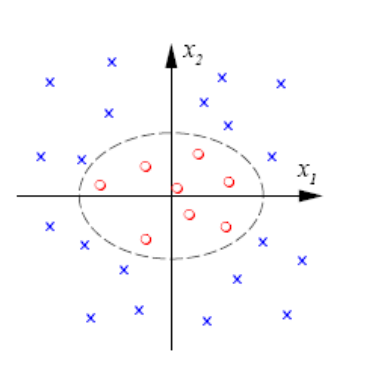
\includegraphics[scale=0.4]{kernel_input.png}
			\captionof{figure}{Input space}
		\end{minipage}
		\begin{minipage}{0.48\linewidth}
			\centering
			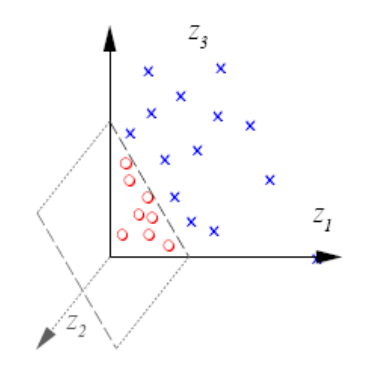
\includegraphics[scale=0.4]{kernel_feature.png}
			\captionof{figure}{Feature space}
		\end{minipage}
	\end{center}
\end{example}
Dato che lavorare con feature space di dimensioni maggiori implica aumentare la complessità del modello e rischiare \textit{overfitting}, usiamo il metodo del \textbf{Kernel} che invece gestisce il feature space tramite la regolarizzazione del modello e che rende quindi la complessità dipendente dal margine, e quindi ridotta.\\
Nell'SVM non è necessario calcolare il vettore $\mathbf{w}$ e di conseguenze nemmeno il prodotto $\mathbf{x}_p^T\mathbf{x}$. Inoltre neanche calcolare direttamente $\phi$. È sufficiente utilizzare il Kernel:
\begin{equation}
	h(\mathbf{x})=sign\bigg(\sum_{p\in SV}\alpha_p y_p K(\mathbf{x}_p,\mathbf{x})\bigg)
\end{equation}
\begin{definition}[Kernel]
	Un kernel $k: \mathbb{R}^n \times \mathbb{R}^n \to \mathbb{R}^n$ è una funzione tale che uno spazio di Hilbert $X$ e una funzione $\phi : \mathbb{R}^n\to X$ esistano con:
	\begin{equation}
		k(\mathbf{x}_i, \mathbf{x}_j)=\phi(\mathbf{x_i})^T\phi(\mathbf{x}_j)
	\end{equation}
\end{definition}
\begin{example}
	L'esempio \ref{example:kernel} può essere calcolato tramite il Kernel in 2 dimensioni invece che in 3:
	\begin{equation*}
		\phi(\mathbf{x_i})^T\phi(\mathbf{x}_j) = (\mathbf{x}_i, \mathbf{x}_j)^2 = K(\mathbf{x}_i, \mathbf{x}_j)
	\end{equation*}
\end{example}
\subsubsection{Kernel conosciuti}
Di seguito alcuni dei Kernel più famosi e utilizzati.
\begin{definition}[Lineare]
	\begin{equation}
		K(\mathbf{x}_i, \mathbf{x}_j) = \mathbf{x}_i^T \mathbf{x}_j
	\end{equation}
	Mappa $\phi: \mathbf{x}\to \phi(\mathbf{x})$, dove $\phi(\mathbf{x})$ è $\mathbf{x}$ stesso.
\end{definition}

\begin{definition}[Polinomiale]
	Data una potenza $p$:
	\begin{equation}
		K(\mathbf{x}_i, \mathbf{x}_j) = (1+\mathbf{x}_i^T \mathbf{x}_j)^k
	\end{equation}
	Mappa $\phi: \mathbf{x}\to \phi(\mathbf{x})$, dove $\phi(\mathbf{x})$ ha un numero di dimensioni esponenziali in $k$.
\end{definition}

\begin{definition}[Radial-basis function]
	Tramite la Gaussiana.
	\begin{equation}
		K(\mathbf{x}_i, \mathbf{x}_j) = e^{-\frac{\lvert\lvert \mathbf{x}_i - \mathbf{x}_j\rvert \rvert^2}{2\sigma^2}}
	\end{equation}
	Mappa $\phi: \mathbf{x}\to \phi(\mathbf{x})$, dove $\phi(\mathbf{x})$ è di dimensioni infinite. \\
	Utilizza l'iperparametro $\sigma$. Se questo è piccolo, i pattern sono considerati simili solo se molto vicini e di conseguenza il classificatore restituisce la classe del punto più vicino. Può essere molto potente ma è anche soggetto a \textbf{overfitting}.
\end{definition}

\begin{observation}
	Bisogna stare attenti alla scelta degli iperparametri per evitare \textbf{overfitting} e sfruttando anche le tecniche di validazione precedentemente descritte.
\end{observation}